\documentclass[11pt]{article}
\usepackage{enumitem}
\usepackage{listings}
\usepackage{tikz}
\usepackage{url}
%\usepackage{algorithm2e}
\usetikzlibrary{arrows,automata,shapes}
\tikzstyle{block} = [rectangle, draw, fill=blue!20, 
    text width=5em, text centered, rounded corners, minimum height=2em]
\tikzstyle{bt} = [rectangle, draw, fill=blue!20, 
    text width=4em, text centered, rounded corners, minimum height=2em]

\lstset{ %
language=Java,
basicstyle=\ttfamily,commentstyle=\scriptsize\itshape,showstringspaces=false,breaklines=true,numbers=left}

\newtheorem{defn}{Definition}
\newtheorem{crit}{Criterion}

\newcommand{\handout}[5]{
  \noindent
  \begin{center}
  \framebox{
    \vbox{
      \hbox to 5.78in { {\bf Software Testing, Quality Assurance and Maintenance } \hfill #2 }
      \vspace{4mm}
      \hbox to 5.78in { {\Large \hfill #5  \hfill} }
      \vspace{2mm}
      \hbox to 5.78in { {\em #3 \hfill #4} }
    }
  }
  \end{center}
  \vspace*{4mm}
}

\newcommand{\lecture}[4]{\handout{#1}{#2}{#3}{#4}{Lecture #1}}
\topmargin 0pt
\advance \topmargin by -\headheight
\advance \topmargin by -\headsep
\textheight 8.9in
\oddsidemargin 0pt
\evensidemargin \oddsidemargin
\marginparwidth 0.5in
\textwidth 6.5in

\parindent 0in
\parskip 1.5ex
%\renewcommand{\baselinestretch}{1.25}

\begin{document}

\lecture{6 --- January 16, 2017}{Winter 2017}{Patrick Lam}{version 2}

\paragraph{Last time.} We discussed benefits of exploratory testing 
and a sketch of how to do it. We also started to do a case study of
WaterlooWorks.

\section*{Source Code Coverage Criteria}
We alluded to statement coverage and branch coverage.  It is possible
to evaluate these criteria directly on the source code, but better to
use a sensible intermediate representation.  The fundamental graph for
source code is the \emph{Control-Flow Graph} (CFG), which originates
from compilers.

\begin{itemize}
\item CFG nodes: a node represents zero or more statements;
\item CFG edges: an edge $(s_1, s_2)$ indicates that $s_1$ may
  be followed by $s_2$ in an execution.
\end{itemize}

\paragraph{Example.} Consider the following code.

\begin{lstlisting}
  x = 5;
  for (z = 2; z < 17; z++)
    print(x);
\end{lstlisting}

Recall the steps in compilation:
\begin{itemize}
\item lexing: input = stream of characters, output = stream of tokens (if, while, strings)
\item parsing: input = stream of tokens, output = concrete syntax tree
\item construction of Abstract Syntax Tree (AST): cleans up the concrete syntax tree
\item conversion to Control Flow Graph: input = AST, output = CFG
\item optimizations: input = CFG, output = CFG
\item convert to bytecode/machine code: input = CFG, output = bytecode/machine code
\end{itemize}

The Abstract Syntax Tree corresponding to the example code might look like this:

\begin{center}
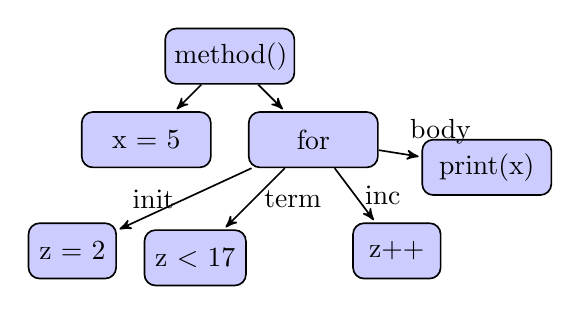
\begin{tikzpicture}[->,>=stealth',shorten >=1pt,auto,node distance=1.5cm,
                    semithick,initial text=]

  \node[bt]           (1) {method()};
  \node[bt]           (2) [below left of=1] {x = 5};
  \node[bt]           (3) [below right of=1] {for};
  \node[bt]           (4) [right of=3,xshift=2em,yshift=-1em] {print(x)};
  \node[bt, text width=2.5em]           (5) [below left of=3,xshift=-2cm,yshift=-1em] {z = 2};
  \node[bt, text width=3em]           (6) [below of=3,xshift=-1.5cm] {z $<$ 17};
  \node[bt, text width=2.5em]           (7) [below right of=3,yshift=-1em] {z++};

  \path (1) edge node {} (2)
  (1) edge node {} (3)
  (3) edge node {body} (4)
  (3) edge node[left] {init} (5)
  (3) edge node[right] {term} (6)
  (3) edge node[right] {inc} (7);
\end{tikzpicture}
\end{center}

\paragraph{From ASTs to CFGs.}

We can convert the Abstract Syntax Tree into the following Control Flow Graph (and we'll see how to do so in Lecture 7).
\begin{center}
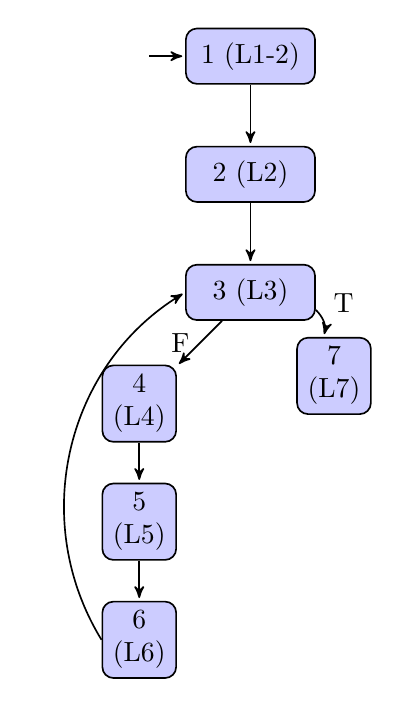
\begin{tikzpicture}[->,>=stealth',shorten >=1pt,auto,node distance=1.5cm,
                    semithick,initial text=]

  \node[initial,bt]   (1)                     {1 (L1-2)};
  \node[bt]           (2) [below of=1]        {2 (L2)};
  \node[bt]           (3) [below of=2] {3 (L3)};
  \node[bt, text width=2em]           (4) [below left of=3,xshift=-1em,yshift=-1em] {4 (L4)};
  \node[bt, text width=2em]           (5) [below of=4,yshift=0em] {5 (L5)};
  \node[bt, text width=2em]           (6) [below of=5,yshift=0em] {6 (L6)};
  \node[bt, text width=2em]           (7) [below right of=3] {7 (L7)};

  \path (1) edge node {} (2)
        (2) edge node {} (3)
        (3) edge node[left] {F} (4)
            edge [bend left] node {T} (7)
        (4) edge node {} (5)
        (5) edge node {} (6)
        (6.west) edge [bend left=45] node {} (3.west);
\end{tikzpicture}
\end{center}

\paragraph{From CFG to low-level code.}
And we can convert the CFG into the following low-level code:
\begin{lstlisting}
    x = 5
    z = 2
q0: if (z < 17) goto q1
    z = z + 1
    print (x)
    goto q0
q1: nop
\end{lstlisting}

\end{document}
